\Exhibit{GitCommit}{%
    Скриншот справки GitHub, объясняющий, что такое коммит%
}

Это начало справочной страницы GitHub, объясняющий,
что коммит это

\ParagraphQuote{%
    как снимок вашего репозитория.
    Коммиты это снимки всего вашего репозитория в определённое время.
    Рекомендуется делать новые коммиты часто, основываясь на логических единицах изменений.
    Со временем коммиты должны рассказывать историю развития вашего репозитория
    и то, как он стал таким, каким он является сейчас.%
}

Это доказывает, что количество коммитов -- это метрика активности разработчиков на проекте,
что коррелировано с важностью проекта.

\begin{center}
    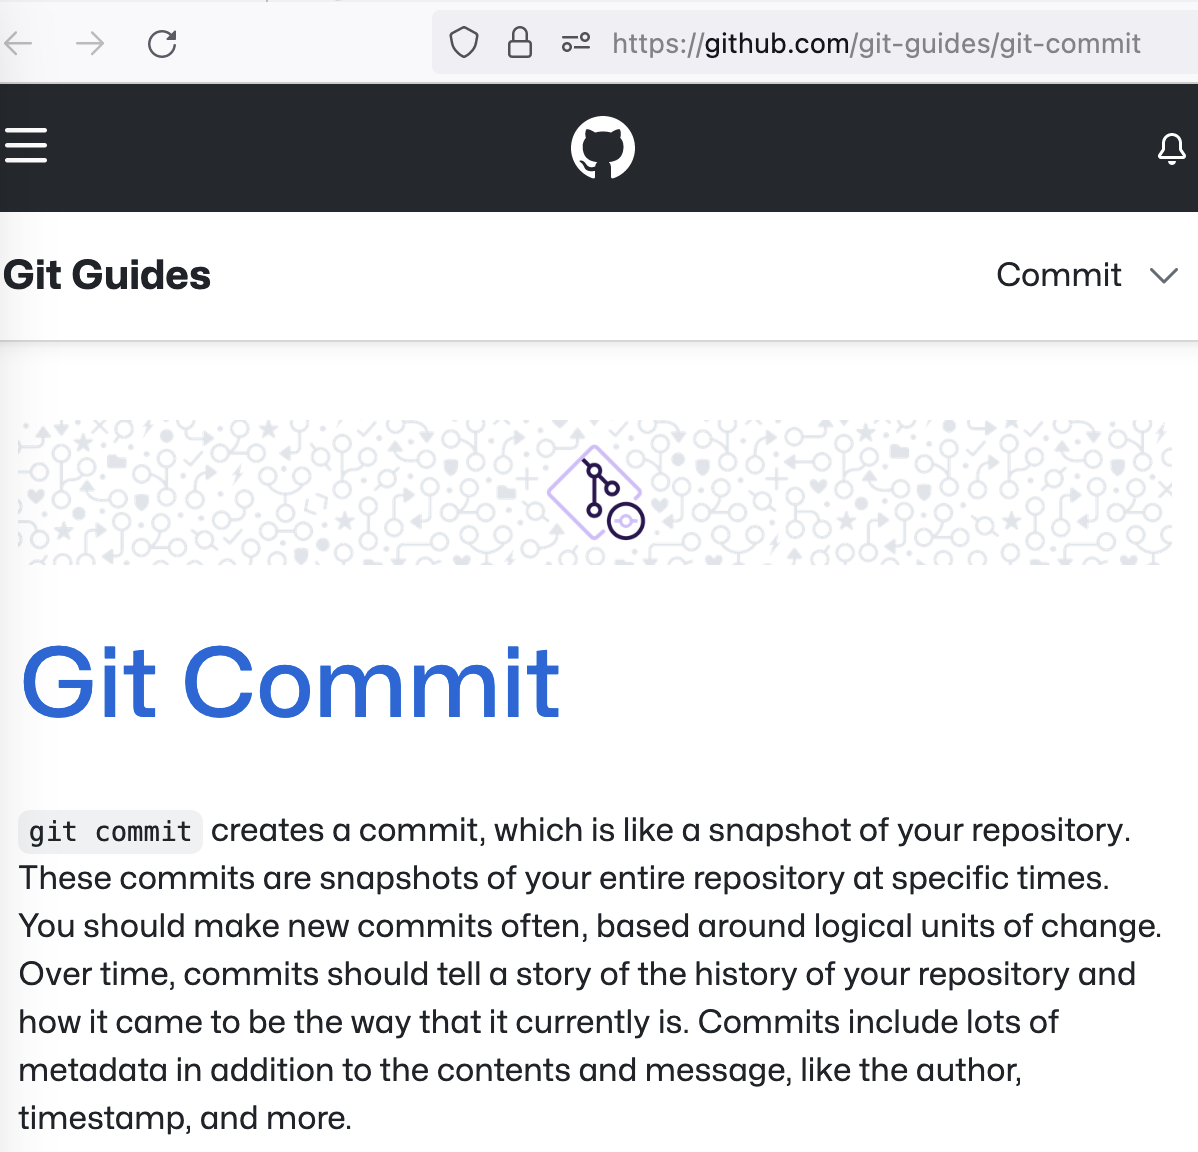
\includegraphics[width=35em]{git-commit}
\end{center}

\pagebreak
